\documentclass[a4paper, english, 12pt, reqno, draft]{amsart}

% ---------------------------------------------------------------------------

% Usepackages recommended in mcom-l-template.tex if needed.

\usepackage{amssymb}
% \usepackage{graphicx}
% \usepackage[cmtip,all]{xy}

% ---------------------------------------------------------------------------

% Usepackages inserted by authors.

\usepackage[english]{babel}
\usepackage[utf8]{inputenc}
\usepackage{tikz,tikzscale}
\tikzset{>=latex}
\usepackage{xcolor}
\usepackage{enumerate}
\usepackage{booktabs,multirow}
\usepackage{amsfonts}
\usepackage{dsfont}

%%%%%%%%%% Packages to help editing %%%%%%%%%%
\usepackage[notref,notcite]{showkeys} % Show labels.
\usepackage[mode=multiuser]{fixme} % Provide note, warning, error, fatal.
\FXRegisterAuthor{gk}{envgk}{GK}
\FXRegisterAuthor{ar}{envar}{AR}
\FXRegisterAuthor{ss}{envss}{SS}
\fxusetheme{color}

% ---------------------------------------------------------------------------

% Theorems in the AMS style.

\newtheorem{theorem}{Theorem}[section]
\newtheorem{lemma}[theorem]{Lemma}
\newtheorem{corollary}[theorem]{Corollary}

\theoremstyle{definition}
\newtheorem{definition}[theorem]{Definition}
\newtheorem{example}[theorem]{Example}
\newtheorem{exercise}[theorem]{Exercise}

\theoremstyle{remark}
\newtheorem{remark}[theorem]{Remark}

\numberwithin{equation}{section}

% ---------------------------------------------------------------------------

% Newcommands by the authors.

\newcommand{\hyperHDG}{{\fontfamily{pzc}\selectfont \texttt{Hy}\hspace{-1.5pt}perHDG }}

\newcommand{\graph}{\ensuremath{\mathcal G}}
\newcommand{\setEdge}{\ensuremath{\mathcal E}}
\newcommand{\setNode}{\ensuremath{\mathcal N}}
\newcommand{\setNodeDir}{\ensuremath{\setNode_\textup D}}
\newcommand{\setNodeNeu}{\ensuremath{\setNode_\textup N}}
\newcommand{\setNodeInt}{\ensuremath{\setNode_\textup I}}
\newcommand{\edge}{\ensuremath{E}}
\newcommand{\node}{\ensuremath{N}}

\newcommand{\Graph}{\ensuremath{\boldsymbol{\mathcal G}}}
\newcommand{\SetEdge}{\ensuremath{\boldsymbol{\mathcal E}}}
\newcommand{\SetNode}{\ensuremath{\boldsymbol{\mathcal N}}}
\newcommand{\SetNodeDir}{\ensuremath{\SetNode_\textup D}}
\newcommand{\SetNodeNeu}{\ensuremath{\SetNode_\textup N}}
\newcommand{\SetNodeInt}{\ensuremath{\SetNode_\textup I}}
\newcommand{\Edge}{{\ensuremath{\boldsymbol E}}}
\newcommand{\RefEdge}{{\ensuremath{\widehat{\boldsymbol e}}}}
\newcommand{\LocEdge}{{\ensuremath{\boldsymbol e}}}
\newcommand{\Node}{{\ensuremath{\boldsymbol N}}}

\newcommand{\locDim}{\ensuremath{\mathfrak d}}
\newcommand{\globDim}{\ensuremath{\mathfrak D}}

\newcommand{\Der}{\ensuremath{\textup d_\Edge}}
\newcommand{\Nabla}{\ensuremath{\nabla_\Edge}}
\newcommand{\Div}{\ensuremath{\Nabla\!\cdot\!}}
\newcommand{\tangent}{\ensuremath{{\boldsymbol T}}}
\newcommand{\Normal}{\ensuremath{\mathfrak n_\Edge}}
\newcommand{\NormalOuter}{\ensuremath{\mathfrak n^\perp_\Edge}}
\newcommand{\RefNormal}{\ensuremath{\mathfrak n_\RefEdge}}
\newcommand{\LocNormal}{\ensuremath{\mathfrak n_\LocEdge}}
\newcommand{\jump}[1]{{[\![ #1 ]\!]}}
\newcommand{\diffeo}{\ensuremath{\Phi}}
\newcommand{\tangentMapping}{\ensuremath{\Phi_{\tangent(x)}}}
\newcommand{\orthProj}{\ensuremath{\Pi_{\tangent(x)}}}
\newcommand{\der}{\ensuremath{\textup D}}
\newcommand{\funcDet}{\ensuremath{g}}
\newcommand{\matQ}{\ensuremath{Q}}
\newcommand{\matR}{\ensuremath{R}}
\newcommand{\basis}{\ensuremath{\mathcal B}}
\newcommand{\unity}{\ensuremath{\mathds 1}}

\newcommand{\IN}{\ensuremath{\mathbb N}}
\newcommand{\IR}{\ensuremath{\mathbb R}}

\newcommand{\skeletal}{\ensuremath{\Sigma}}
\newcommand{\skeletalSpace}{\ensuremath{M}}
\newcommand{\discElementSpace}{\ensuremath{V}}
\newcommand{\polynomials}{\ensuremath{\mathcal P}}

\renewcommand{\vec}[1]{\ensuremath{\boldsymbol{#1}}}
\DeclareMathAlphabet{\mathbfsf}{\encodingdefault}{\sfdefault}{bx}{n}
\newcommand{\vecc}[1]{\ensuremath{\mathbfsf{#1}}}
\newcommand{\Nu}{\ensuremath{\vec \nu}}
\newcommand{\dx}{\ensuremath{\, \textup d x}}
\newcommand{\dy}{\ensuremath{\, \textup d y}}
\newcommand{\ds}{\ensuremath{\, \textup d \sigma}}
\newcommand{\localU}{\ensuremath{\mathcal U}}
\newcommand{\localQ}{\ensuremath{\vec{\mathcal Q}}}
\newcommand{\range}{\ensuremath{\mathcal R}}

\newcommand{\code}[1]{\texttt{#1}}

\newcommand{\longDef}{\ensuremath{u}}
\newcommand{\crossDef}{\ensuremath{w}}
\newcommand{\torsion}{\ensuremath{\varphi}}
\newcommand{\force}{\ensuremath{q}}
\newcommand{\momentum}{\ensuremath{m}}
\newcommand{\crossSect}{\ensuremath{\mathcal A}}

% ---------------------------------------------------------------------------

% Make paragraph heading being small capitals!

\makeatletter
\def\paragraph{\@startsection{paragraph}{4}%
  \z@\z@{-\fontdimen2\font}%
  {\normalfont\scshape}}
\makeatother

% ---------------------------------------------------------------------------

% Usepackage hyperref is the last to be added!

\usepackage[colorlinks = true, linkcolor = blue, citecolor = blue, urlcolor = blue]{hyperref}

% ---------------------------------------------------------------------------

% Document head as described in the template.

\begin{document}

\title[\hyperHDG --- HDG on hypergraphs]{\hyperHDG --- Hybrid disontinuous Galerkin methods for PDEs on hypergraphs} 

\author{Andreas Rupp}
\address{Interdisciplinary Center for Scientific Computing (IWR), Heidelberg University, Mathematikon, Im Neuenheimer Feld 205, 69120 Heidelberg, Germany}
% \curraddr{}
\email{andreas.rupp@fau.de, andreas.rupp@uni-heidelberg.de}
\thanks{This work is supported by the Deutsche Forschungsgemeinschaft (DFG, German Research Foundation) under Germany's Excellence Strategy EXC 2181/1 - 390900948 (the Heidelberg STRUCTURES Excellence Cluster).}

\author{Guido Kanschat}
\address{Interdisciplinary Center for Scientific Computing (IWR) and Mathematics Center Heidelberg (MATCH), Heidelberg University, Mathematikon, Im Neuenheimer Feld 205, 69120 Heidelberg, Germany}
% \curraddr{}
\email{kanschat@uni-heidelberg.de}
% \thanks{}

\subjclass[2010]{\textcolor{red}{TODO}}

\date{\today}

% \dedicatory{}

\begin{abstract}
 \textcolor{red}{\textsc{Todo!}} 
 \\[1ex] \noindent \textsc{Keywords.}
 \textcolor{red}{TODO!}
\end{abstract}
% 
\allowdisplaybreaks
\maketitle
% 

\begin{envarnote}{Editing!}
 Dear all,
 
 since we are quite many people, I have included the usepackage ``fixme''. It provides quite powerful tools for editing text. You can use a note, a warning, an error, or a fatal to indicate things in the text. Using the initials it can be tracked who set a comment. Analogously, it works for warnings, errors, and fatals. Thus, using the command \verb|\arnote{This is a note by Andreas Rupp}| creates a note at the margins, where the ar in arnote stands for Andreas Rupp. Moreover, \verb|\begin{envarnote}{Short description} ..... \end{envarnote}| \linebreak will create a short descripton at the margin and a long text (like this) within the standard text.
\end{envarnote}
% 
\section{Introduction}
% 
\textcolor{red}{TODO!}
% ---------------------------------------------------------------------
\section{Hypergraphs}\label{SEC:hypergraph}
% ---------------------------------------------------------------------
% 
\hyperHDG is a simumlation software to perform numerical experiments on so called hypergraphs. To this end, it is useful to discuss the composition of hypergraphs in some detail. At first, every hypergraph is defined as topological hypergraph, cf. Section. \ref{SEC:hypergraph_topology}. Additionally, a hypergraph may be equipped with a geometry, as illuminated in Section \ref{SEC:hypergraph_geometry}. 
% 
\subsection{Topologic aspects of hypergraphs}\label{SEC:hypergraph_topology}
% 
In the whole manuscript, we consider a \emph{hypergraph} $\graph = (\setNode,\setEdge)$ consisting of a finite set of \emph{hypernodes} $\setNode = \{\node_1, \node_2, \ldots \}$ and a finite set of \emph{hyperedges} $\setEdge = \{\edge_1, \edge_2, \ldots \}$. All hyperedges $\edge \in \setEdge$ can be interpreted as connecting several nodes and, thus, can be written as $\edge \subset \setNode$.

Thus, the topology of a hypergraph $\graph$ is a pair consisting of a set of hyperedges $\setEdge$ and a set of hypernodes $\setNode$. Each hyperedge $\edge \in \setEdge$ is connected to other hyperedges via the set of its adjacent hypernodes. Note that this is exactly the inverted interpretation as compared to the aforementioned definition of a hypergraph, where nodes are interpreted as connected via edges.

\paragraph{Cubic and simplicial hypergraphs, and local dimension $\locDim$}
% 
We will define partial differential equations (PDEs) on hypergraphs. To do so, it helps---but is not necessary---to have an adequate graphical representation of hyperedges. For example, one might try to represent all $\edge \in \setEdge$ as (relatively) open unit hypercubes of dimension $\locDim \in \IN$. A hypergraph, of which all hypereges $\edge = \{ \node_1, \node_2, \ldots, \node_{2\locDim} \}$ consist of exactly $2\locDim$ hypernodes, allows for such a representation of all hyperedges. The hypernodes may then be interpreted as the \emph{faces} (not the vertices) of the hypercubes/hyperedges and the hypergraph is denoted \emph{cubic} of \emph{local dimension} $\locDim$. In this representation, also the hypernodes are supposed to be (relatively) open sets.

Analogously, a hypergraph of which all hyperedges consist of $\locDim+1$ hypernodes is called \emph{simplicial} of local dimension $\locDim$.

\paragraph{Cubic/simplicial (topological) embeddings of hypergraphs to global dimension $\globDim$}
% 
If one wants to represent the whole hypergraph at once (instead of only single hyperedges), an embeddind to an $\globDim$ dimensional space is needed. To allow for an easy notation, we denote by $\Edge \in \SetEdge$ the representation of $\edge \in \setEdge$ as (relatively) open, but smoothly deformed hypercube/simplex, by $\node \in \setNode$ the representation of a hypernode $\Node \in \SetNode$ as (relatively) open (deformed) face, and set $\Graph = (\SetNode, \SetEdge)$. A cubic/simplicial hypergraph can be \emph{topologically embedded} into $\IR^\globDim$ if
% 
\begin{enumerate}
 \item there is a way to assemble all deformed hypercubes/simplices (representing the hyperedges) such that for two different hyperedges $\edge^+ \neq \edge^-$ and two hypernodes $\node^- \neq \node^+$, we have $\Edge^- \cap \Edge^+ = \emptyset$ and $\Node^- \cap \Node^+ = \emptyset$.
 \item in the aforementioned assembly for all $\node \in \setNode$ and $\edge \in \setEdge$: We have $\Node \cap \Edge \neq \emptyset$ if, and only if, $\node \in \edge$.
\end{enumerate}
% 
\paragraph{Examples for cubic hypergraphs}
% 
According to this definition, every graph is both a cubic and a simplicial hypergraph. An illustration which can be interpreted as several hypergraphs---all embedded to $\globDim = 3$---can be found in Figure \ref{FIG:hyG_topo}:
% 
\begin{itemize}
 \item Cubic or simplicial hypergraph of $\locDim = 1$ consisting of twelve hypernodes (vertices) and  twenty hyperedges (lines).
 \item Cubic hypergraph of $\locDim = 2$ consisting of twenty hypernodes (lines) and eleven hyperedges (squares).
 \item Cubic hypergraph of $\locDim = 3$ consisting of eleven hypernodes (squares) and two hyperedges (cubes).
\end{itemize}
% 
\begin{figure}[ht]
 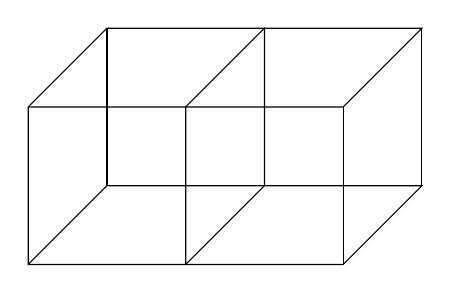
\begin{tikzpicture}
  \draw (0,0) -- (2,0) -- (4,0) -- (5,1) -- (3,1) -- (1,1) -- (0,0) -- (0,2) -- (2,2) -- (4,2) -- (5,3) -- (3,3) -- (1,3) -- (0,2);
  \draw (2,0) -- (3,1) -- (3,3) -- (2,2) -- (2,0);
  \draw (1,1) -- (1,3);
  \draw (4,0) -- (4,2);
  \draw (5,1) -- (5,3);
 \end{tikzpicture}
 \caption{Illustration that can be interpreted as several types of hypergraph topologies.}\label{FIG:hyG_topo}
\end{figure}
% 
\subsection{Geometrical aspects of hypergraphs}\label{SEC:hypergraph_geometry}
% 
Figure \ref{FIG:hyG_topo} already indicates that hypergraphs, especially those with embeddings might be equipped with geometrical information. This specific example indicates that all lines, squares, cubes are of unit size. However, the hypergraph might also have geometrical information that says it looks like in Figure \ref{FIG:hyG_geom}, where the first picture is valid for all $\locDim$ and the second one is only valid for $\locDim = 3$. Note that, all sufaces may also be curved, but we restrict to straight representations, here.
% 
\begin{figure}[ht]
 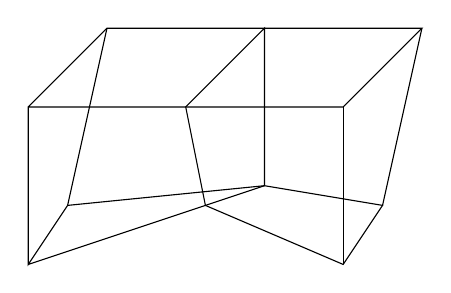
\begin{tikzpicture}
  \draw (0,0) -- (2.25,0.75) -- (4,0) -- (4.5,0.75) -- (3,1) -- (0.5,0.75) -- (0,0) -- (0,2) -- (2,2) -- (4,2) -- (5,3) -- (3,3) -- (1,3) -- (0,2);
  \draw (2.25,0.75) -- (3,1) -- (3,3) -- (2,2) -- (2.25,0.75);
  \draw (0.5,0.75) -- (1,3);
  \draw (4,0) -- (4,2);
  \draw (4.5,0.75) -- (5,3);
 \end{tikzpicture}
 \quad
  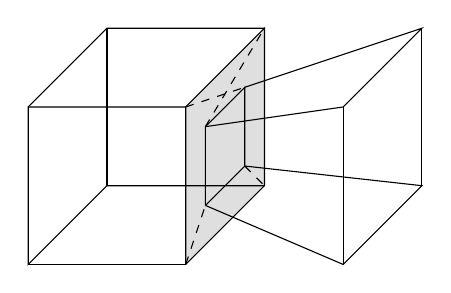
\begin{tikzpicture}
  \path[fill=gray!25] (2,0) -- (3,1) -- (3,3) -- (2,2) -- (2,0);
  \draw (0,0) -- (2,0);
  \draw[dashed] (2,0) -- (2.25,0.75);
  \draw (2.25,0.75)  -- (4,0) -- (5,1) -- (2.75,1.25);
  \draw[dashed] (2.75,1.25) -- (3,1);
  \draw (3,1) -- (1,1) -- (0,0) -- (0,2) -- (2,2);
  \draw (2.25,1.75) -- (4,2) -- (5,3) -- (2.75,2.25); 
  \draw (3,3) -- (1,3) -- (0,2);
  \draw[dashed] (2,2) -- (2.75,2.25);
  \draw[dashed] (2.25,1.75) -- (3,3);
  \draw (2,0) -- (3,1) -- (3,3) -- (2,2) -- (2,0);
  \draw (2.25,0.75) -- (2.75,1.25) -- (2.75,2.25) -- (2.25,1.75) -- (2.25,0.75);
  \draw (1,1) -- (1,3);
  \draw (4,0) -- (4,2);
  \draw (5,1) -- (5,3);
 \end{tikzpicture}
 \caption{Two possible geometrical representation of the hypergraph in Figure \ref{FIG:hyG_topo}. The second one is only valid for $\locDim = 3$---the gray hypernode has different geometrical representations for the two adjacent hyperedges.}\label{FIG:hyG_geom}
\end{figure}

This motivates the following observation: A hypergraph can, beyond its topological information, carry geometrical information. That is, for all hyperedges, there is a geometry prescribed.

This can lead to the case that for one hypernode, different geometries are prescribed as illustrated gray in the right picture of Figure \ref{FIG:hyG_geom}. The hypernode can also be disorted as illustrated by the dashed lines indicating that the two top vertices have to interchange when reinterpreting the node as face of the one or the other hyperedge. This could not be easily illustrated in the picture if the right version of the hypernode was not smaller than the left version. Thus, the hypernode would look as if no reinterpretation is necessary, although in fact, it is.

\paragraph{Embedded hypergraphs}
% 
If the hypergraph can be topologically embedded to dimension $\globDim$ and carries geometrical information for the hyperedges, such that for all hypernodes, there is a unique geometrical description---excluding that the hypernode is disorted or has different shapes for different hyperedges, then the hypergraph can be \emph{topological and geometrical embedded} (for short, just \emph{embedded}) into $\IR^\globDim$. For the representation of the embeddded hypergraph, we also use the notation with the bold symbols.

\paragraph{Smoothness assumptions}
% 
We assume that all hyperedges $\IR^\globDim \supset \Edge \in \SetEdge$ allow for a $C^\infty$ diffeomorphism
% 
\begin{equation*}
 \diffeo_\Edge \colon \; \IR^\locDim \supset \RefEdge ~\mapsto~ \Edge \subset \IR^\globDim,
\end{equation*}
% 
where the reference element $\RefEdge$ is either a unit simplex of a unit hypercube.

Thus, the $\Edge\in \setEdge$ are \emph{Riemannian manifolds}, i.e., they are real, smooth manifolds, and for all $x \in \Edge$, they are equipped with an inner product $(\cdot,\cdot)_{\tangent(x)}$ with respect to the \emph{tangent space} $\tangent(x)[\Edge] \subset \IR^\globDim$ of the manifold $\Edge$ evaluated at point $x$. If no confusion is possible, the expression $[\Edge]$ is dropped. We set the inner product as standard \emph{Euclidean scalar product}
% 
\begin{equation*}
 (a,b)_{\tangent(x)} = (a,b)_{\IR^\globDim} =: (a,b) \qquad \text{ for all } a,b \in \tangent(x) \text{ and } x \in \Edge
\end{equation*}
% 
and define $\| x \|^2 := (x,x)$ for $x \in \IR^\globDim$.

\paragraph{Linear hypergraphs}
% 
A cubic/simplicial hypergraph is called \emph{linear} if all hyperedges $\SetEdge \ni \Edge \subset \IR^\globDim$ can be represented as image of an affine-linear mapping of a (reference) unit hypercube/simplex $\RefEdge \subset \IR^\locDim$. This implies that all faces are straight and that the transformation matrix is square if and only is $\locDim = \globDim$.
% ---------------------------------------------------------------------
\section{Elliptic model equation and interpretation}\label{SEC:model_eq}
% ---------------------------------------------------------------------
% 
Here, we formulate the standard diffusion equation in mixed form defined on a hypergraph $\graph$ that for the moment is assumed to allow an embedding $\Graph$. The differential operators will be rigorously defined in Section \ref{SEC:diff_op}. Thus, for all $\edge \in \setEdge$ we approximate solutions $(u, \vec q)$ of
% 
\begin{subequations}\label{EQ:diffusion_mixed}
\begin{align}
 \Div \vec q & = f && \text{ in } \Edge,\label{EQ:div_is_f}\\
 \tfrac{1}{d} \vec q + \Nabla u & = 0 && \text{ in } \Edge,\label{EQ:primal_dual}
\end{align}
% 
for a given functions $d \ge d_0 > 0$ and $f$. Here, $u$ may be considered as concentration and $\vec q$ as flux of a chemical species diffusing on the hypersurface $\Edge$.

Additionally, we assume that there is a non-empty set $\setNodeDir \subset \setNode$ of Dirichlet hypernodes, a possibly empty set $\setNodeNeu \subset \setNode\setminus \setNodeDir$ of Neumann hypernodes, and the remainder set $\setNodeInt = \setNode \setminus (\setNodeDir \cup \setNodeNeu)$ of interior hypernodes. The following ideas motivate three different types of closing conditions:
% 
\begin{itemize}
 \item On hypernodes of Dirichlet type, the value of function $u$ is prescribed by function $u_\text D$.
 \item On hypernodes of Neumann type, outflow of the whole system/hypergraph with rate $g_\textup N$ is prescribed. The outflow of chemical species with respect to a hyperedge is defined via $\vec q \cdot \Normal$. Here, $\Normal$ is the outward unit normal with respect to the hyperedge, cf. Section \ref{SEC:normals}. Thus the sum of outflows of all hyperedges adjacent to the Neumann node should be equal to $g_\textup N$.
 \item Interior hypernodes are Neumann hypernodes with $g_\textup N \equiv 0$ describing conservation of the chemical species.
\end{itemize}
% 
For PDEs on manifolds or the full space, the sum of outflows of all hyperedges adjacent to a hypernode consists of either one (at the boundary) or two summands and typically is represented by the notion of a \emph{jump} $\jump{\vec q}$, which can be generalized to
% 
\begin{equation*}
 \jump{\vec q}_\Node = \sum^{\edge \in \setEdge}_{\edge \ni \node} \vec q_\Edge \cdot \Normal \quad \text{ with } \quad \vec q_\Edge = \vec q|_\Edge,
\end{equation*}
% 
turning the vector function $\vec q$ to a scalar and being defined for all hyppernodes. The subscript $\Node$ will be dropped if no confusion is possible. Using this generalization, the closing conditions can be formulated into the following equations:
% 
\begin{align}
 u & = u_\textup D && \text{ on } \Node \in \SetNodeDir,\label{EQ:dir_cond}\\
 \jump{\vec q} & = g_\textup N && \text{ on } \Node \in \SetNodeNeu,\label{EQ:neu_cond}\\
 \jump{\vec q} & = 0 && \text{ on } \Node \in \SetNodeInt.\label{EQ:int_cond}
\end{align}
\end{subequations}
% 
Thus, \eqref{EQ:diffusion_mixed} is a direct generalization of the standard diffusion equation in the whole space---even with the same notation---if we manage to find proper direct generalizations of normals and differential operators.
% 
\subsection{The notion of normals}\label{SEC:normals}
% 
In the following, we will define different notions of normals with respect to a hyperedge $\Edge \in \SetEdge$. The simplest type of normal is the \emph{outer normal} $\NormalOuter \in \IR^\globDim$, which is defined via
% 
\begin{equation*}
 \|\NormalOuter(x)\| = 1 \qquad \text{ and } \qquad (\NormalOuter(x), v) = 0 \quad \text{ for all } v \in \tangent(x).
\end{equation*}
% 
The second condition can be abbreviated to $\NormalOuter(x) \perp \tangent(x)$. For each point $x \in \Edge$ there either exist no ($\locDim = \globDim$), two ($\locDim = \globDim - 1$) or infinitely many outer normals.

Additionally, for $x \in \partial \Edge$, we define the \emph{inner normal} $\Normal \in \IR^\globDim$ as unique, outward pointing vector with
%
\begin{equation}\label{EQ:inner_const}
 \| \Normal \| = 1, \qquad \Normal \in \tangent(x), \qquad \Normal \perp \tangent(x) [\partial \Edge]
\end{equation}

Considering the the reference element $\RefEdge \subset \IR^\locDim$, we define the \emph{reference normal} $\RefNormal \subset \IR^\locDim$ on its boundary as as the unit outward pointing normal of the reference edge. Furthermore assuming that $\der \diffeo_\Edge(x) = \matQ_\Edge \matR_\Edge$ is an $\matQ \matR$ decomposition (a specific normalized one will be used in Section \ref{SEC:HDG_loc_prob}), we define the \emph{local normal} $\LocNormal \in \IR^\locDim$ as outward unit normal of
% 
\begin{equation*}
 \LocEdge := \widehat \matR_\Edge \RefEdge,
\end{equation*}
% 
where $\widehat \matR_\Edge \in \IR^{\locDim,\locDim}$ is the upper left $\locDim \times \locDim$ block of $\matR_\Edge$ (containing the non-zero entries). Note that if $\widehat \LocNormal \in \IR^\globDim$ is the vector containing $\LocNormal(\hat x)$ and zeros below its entries, and $\hat x = \diffeo^{-1}_\Edge x \in \partial \RefEdge$, we have
% 
\begin{equation}\label{EQ:def_inner}
 \matQ^T_\Edge \Normal(x) = \widehat \LocNormal.
\end{equation}
% 
This equation actually is used to determine inner normals, since constructing an outward pointing vector sufficing \eqref{EQ:inner_const} is not a trivial task.
% 
\subsection{Differential operators on hyperedges}\label{SEC:diff_op}
% 
Consider the smooth function $f: \Edge \to \IR$. Its \emph{directional derivative} in $x \in \Edge$ and direction $v \in \tangent(x)$ is defined as
% 
\begin{equation}\label{EQ:direc_der}
 [\Der f(x)](v) ~:=~ \frac{\textup d}{\textup d \tau} (f \circ \gamma)(\tau)|_{\tau = 0}
\end{equation}
% 
for any smooth curve $\gamma: (-1,1) \to \Edge$ with $\gamma(0) = x$ and $\gamma'(0) = v$.

Accordingly, the \emph{derivative} is defined as
% 
\begin{equation*}
 \Der f(x) \colon \tangent(x) \to \IR, \qquad \text{ \eqref{EQ:direc_der} holds for all $v \in \tangent(x)$.}
\end{equation*}
% 
Thus, $\Der f(x) \in \tangent^\star(x)$ which is the dual space of $\tangent (x)$ and there is a well-defined mapping $\Der f \colon \Edge \to \tangent^\star(x)$. According to Riesz representation theorem, there is a unique \emph{gradient} $\Nabla f \colon \Edge \to \tangent(x)$ with
% 
\begin{equation*}
 (\Nabla f(x), v) = [\Der f(x)](v) \qquad \forall x \in \Edge, \forall v \in \tangent(x).
\end{equation*}
% 
In terms of muscial isomorphisms, that is
% 
\begin{equation*}
 \Nabla f = (\Der f)^\sharp \qquad \text{ and } \qquad \Der f = (\Nabla f)^\flat.
\end{equation*}

The definition of the \emph{divergence} of a smooth vector function $\vec f \colon E \to \tangent(x)$ can be done using an orthonormal basis $\basis$ of $\tangent(x)$---which contains $\locDim$ elements---and setting
% 
\begin{equation*}
 \Div \vec f: \Edge \to \IR, \qquad [\Div \vec f](x) = \sum_{b \in \basis} [\Der (f, b)_{\tangent(x)} (x)](b).
\end{equation*}
% 
% ---------------------------------------------------------------------
\section{HDG method on hypergraphs}
% ---------------------------------------------------------------------
%
In this section, we discuss the HDG method applied to the diffusion equation on a hypergraph. Thus, we first formulate the method in Section \ref{SEC:HDG_form} and discuss implementation aspects of local problems (including transformation rules for the necessary integrals and differential operators) in Section \ref{SEC:HDG_loc_prob}. At last, we describe an efficient way of solving the global system of equations arising from the HDG discretizaion in Section \ref{SEC:glob_system}.
% 
\subsection{HDG formulation}\label{SEC:HDG_form}
% 
Let $p\ge 1$ and $\polynomials_p$ be the space of (multivariate)
polynomials of degree up to $p$. Then, we define the space of piecewise polynomials on the skeleton $\skeletal := \bigcup_{\Node \in \SetNode} \Node$ by
% 
\begin{gather}\label{EQ:skeletal_space}
 \skeletalSpace := \left\{ \lambda \in L^2(\skeletal) \;\middle|\;
 \begin{array}{r@{\,}c@{\,}ll}
  \lambda_{|\Node} &\in& \polynomials_p & \forall \Node \in \SetNode\\
  \lambda_{|\Node} &=& 0 & \forall \Node \in \SetNodeDir    
 \end{array}
 \right\}.
\end{gather}
% 
The HDG method involves a local solver on each mesh hyperege
$\Edge \in \SetEdge$, producing hyperedge-wise approximations $U_\Edge \in V_\Edge$ and and $\vec Q_\Edge \in \vec W_\Edge$ of the functions $u$ and $\vec q$ in equation~\eqref{EQ:diffusion_mixed}, respectively. We choose $V_\Edge = \polynomials_p$. Then, choosing
$\vec W_\Edge = \polynomials_p^d$ yields the so called hybridizable local discontinuous Galerkin (LDG-H) scheme. We will also use the concatenations of the spaces $V_\Edge$ and $\vec W_\Edge$, respectively, as a function space on $\Omega$, namely
\begin{gather}\label{EQ:dg_spaces}
 \begin{aligned}
  \discElementSpace &:=\bigl\{ v \in L^2(\Omega) & \big|\;v_{|\Edge} &\in V_\Edge, &\forall \Edge &\in \SetEdge \bigr\},\\
  \vec W &:=\bigl\{ \vec q \in L^2(\Omega;\mathbb R^d) & \big|\;\vec q_{|\Edge} &\in \vec W_\Edge, &\forall \Edge &\in \SetEdge \bigr\}.
 \end{aligned}
\end{gather}
% 
The HDG scheme for~\eqref{EQ:diffusion_mixed} on a mesh $\Graph$
consists of the local solver and a global coupling equation. The local solver is defined hyperedge-wise by a weak formulation
of~\eqref{EQ:diffusion_mixed} in the discrete spaces
$V_\Edge \times \vec W_\Edge$ and defining suitable numerical traces and fluxes. Namely, given $\lambda \in \skeletalSpace$ find $U_\Edge \in V_\Edge$ and $\vec Q_\Edge \in \vec W_\Edge$ , such that
% 
\begin{subequations}\label{EQ:hdg_scheme}
 \begin{align}
  \int_\Edge \tfrac{1}{d} \vec Q_\Edge \cdot \vec p \dx - \int_\Edge U_\Edge \Div \vec p \dx & = - \int_{\partial \Edge} \lambda \vec p \cdot \Normal \ds \label{EQ:hdg_primary}\\
  - \int_\Edge \vec Q_\Edge \cdot \Nabla v \dx  + \int_{\partial \Edge} ( \vec Q_\Edge \cdot \Normal + \tau  U_\Edge ) v \ds
  & = \tau \int_{\partial \Edge} \lambda v \ds \label{EQ:hdg_flux}
 \end{align}
\end{subequations}
% 
hold for all $v \in V_\Edge$, and all $\vec p \in \vec W_\Edge$, and for all $\Edge \in \SetEdge$. Here, $\tau > 0$ is the penalty coefficient. While the local solvers are implemented hyperedge by hyperedge, it is helpful for the analysis to combine them by concatenation. Thus, the local solvers define a mapping
% 
\begin{gather}
 \begin{split}
  \skeletalSpace & \to \discElementSpace \times \vec W\\
  \lambda &\mapsto (\localU \lambda, \localQ \lambda),
 \end{split}
\end{gather}
% 
where for each hyperedge $\Edge \in \SetEdge$ holds $\localU \lambda = U_\Edge$ and $\localQ \lambda = \vec Q_\Edge$. In the same way, we define operators $\localU u_\textup D$ and $ \localQ u_\textup D$, where in \eqref{EQ:hdg_scheme}, $\lambda$ is replaced by $u_\textup D$ on Dirichlet nodes, and by zero otherwise. Analogously, we set  $\localU f$ and $ \localQ f$ for
$f\in L^2(\bigcup_{\Edge \in \SetEdge} \Edge)$, where now the local solutions are defined by the system
% 
\begin{subequations}\label{EQ:hdg_f}
 \begin{align}
  \int_\Edge \tfrac{1}{d} \vec Q_\Edge \cdot \vec p \dx - \int_\Edge U_\Edge \Div \vec p \dx & = 0 \label{EQ:hdg_f_primary}\\
  - \int_\Edge \vec Q_\Edge \cdot \Nabla v \dx  + \int_{\partial \Edge} ( \vec Q_\Edge \cdot \Normal + \tau U_\Edge ) v \ds & =  \int_{\Edge} f v \dx\label{EQ:hdg_f_flux}
 \end{align}
\end{subequations}

Once $\lambda$ has been computed, the HDG approximation
to \eqref{EQ:diffusion_mixed} on $\Graph$ will be computed as
% 
\begin{gather}
  \begin{split}
    U &= \localU \lambda + \localU u_\textup D + \localU f\\
    \vec Q &= \localQ \lambda + \localQ u_\textup D + \localQ f
  \end{split}
\end{gather}

The global coupling condition is derived through a discontinuous
Galerkin version of mass balance and reads: Find
$\lambda \in \skeletalSpace$, such that for all
$ \mu \in \skeletalSpace$
% 
\begin{equation}
 \sum_{\edge \in \setEdge} \sum^{\node \in \setNode \setminus \setNodeDir}_{\node \in \edge} \int_\Node \left[ \vec Q \cdot \Normal + \tau (U - \lambda) \right] \mu \ds = \sum_{\node \in \setNodeNeu} \int_\Node g_\textup N \mu \ds.\label{EQ:hdg_global}
\end{equation}
% 
\subsection{Implementation aspects of local problems}\label{SEC:HDG_loc_prob}
% 
Trying to implement local problems \eqref{EQ:hdg_scheme} or \eqref{EQ:hdg_f}, we need efficient ways to evaluate integrals with respect to hyperedges or hypernodes, and the differential operators of Section \ref{SEC:diff_op}. We start with an improved way of formulating integrals of the type
% 
\begin{equation}
 \int_\Edge f \ds = \int_\RefEdge \left[f \circ \diffeo^{-1}_\Edge\right] \underbrace{ \sqrt{\det[(\der\diffeo)^T \der \diffeo]} }_{ =: \funcDet }\dx,
\end{equation}
% 
where $\der$ denotes the standard total derivative and $\funcDet$ is the functional determinant. Thus, $g$ can be interpreted as generalization of the determinant of $\der\diffeo$, which in general is not a square matrix. However, via $\matQ\matR$ decomposition
% 
\begin{equation}\label{EQ:QR_decomp}
 \der\diffeo = \matQ_\Edge \matR_\Edge, \qquad \der\diffeo \in \IR^{\globDim,\locDim}, \, \matQ \in \IR^{\globDim,\globDim}, \, \matR \in \IR^{\globDim,\locDim},
\end{equation}
% 
where $\matQ_\Edge$ is an orthogonal (square) matrix with with $\det \matQ_\Edge = 1$ and $\matR$ is an upper triangular matrix with $(\matR_\Edge)_{i,i} \ge 0$ for all $i \ge 2$.  $(\matR_\Edge)_{1,1}$ should be non-negative if this is possible without violating the aforementioned conditions. Note that all enries $(\matR_\Edge)_{i,j} = 0$, for $i > \locDim$ or $j > \locDim$. Thus, we can equivalently calculate
% 
\begin{equation}\label{EQ:det_gen}
 \funcDet = \left| \det\der\diffeo \right|, \qquad \det\der\diffeo := \prod_{i=1}^\locDim (\matR_\Edge)_{i,i}.
\end{equation}
% 
Note that from this representation, we can also deduce whether $\diffeo$ preserves orientation, i.e., $(\matR_\Edge)_{1,1} \ge 0 \Leftrightarrow \det\der\diffeo \ge 0$, or changes orientation, i.e., $(\matR_\Edge) \ge 0$. Thus, we have that $\det$ from \eqref{EQ:det_gen} is a direct generalization of the standard determinant and gives the same value for square matrices. Thus, it carries the same notation. Analogous considerations allow to evaluate integrals with respect to hypernodes.

For the transformation of gradient and divergence, we will investigate the transformation of directional derivatives, first. The general formulas can then be constructed by combining the different directional derivatives, but are not used for implementation, where all directional derivatives are treated independently. We have that
% 
\begin{align*}
 [\der_\RefEdge (f \circ \diffeo) (\hat x)](\hat v) ~=~ & \frac{\textup d}{\textup d \tau} (f \circ \diffeo \circ \gamma) (\tau)|_{\tau = 0} \\
 ~=~ & [\der_{\diffeo \circ \gamma} f ((\diffeo\circ\gamma) (0))] \cdot [\der_{\gamma} \diffeo(\gamma (0))] \cdot \der_{\tau} \gamma(0)\\
 ~=~ & [\Der f (x)] \left( \der_{\hat v} \diffeo(\hat x) \right) ~=~[\Der f (x)] (v)
\end{align*}
% 
for $\gamma(0) = \hat x := \diffeo^{-1}_\Edge x$ and $\gamma'(0) = \hat v$ with $v = (\der_{\hat x} \diffeo_\edge(\hat x))\hat v$ (matrix--vector product), and the hat indicating that functions or operators live on the reference element. Here, also $\der_{\hat v} \diffeo(\hat x)$ is the directional derivative and $\cdot$ indicates just a product and that not application of a function is meant. This need not be the scalar product, here. Thus, we formally recover
% 
\begin{equation*}
 [\Der f (x)] (v) = [\der_\RefEdge (f \circ \diffeo) (\hat x)]([\der_{\hat x} \diffeo_\edge(\hat x)]^{-1} v).
\end{equation*}
% 
This is a generalization of the standard transformation formula for directional derivatives. However, the inverse is not well-defined, since the the derivative of $\diffeo$ cannot be assigned to a square matrix. Nonetheless, due to $v \in \range (\der_{\hat x} \diffeo_\edge(\hat x))$, it is well-defined in the sense of a mapping.

To gain an efficient implementation for the gradient and the divergence, we next define a local, orthonormal coordinate system on the tangent $\tangent(x)$ by using the first $\locDim$ column vectors of $\matQ$ from \eqref{EQ:QR_decomp}. This basis, for the sake of implementation, is also used as the basis for the divergence, as described in Section \ref{SEC:diff_op}: $\basis = \{b_1, \ldots, b_\locDim\}$. Thus, we can write
% 
\begin{align*}
 [\Der f (x)] (b_j) ~=~ & [\der_\RefEdge (f \circ \diffeo) (\hat x)]([\der_{\hat x} \diffeo_\edge(\hat x)]^{-1} b_j)\\
 ~=~ & [\der_\RefEdge (f \circ \diffeo) (\hat x)] (\matR^{-1}_\Edge \matQ^T_\Edge b_j)\\
 ~=~ & [\der_\RefEdge (f \circ \diffeo) (\hat x)] (r_j)
\end{align*}
% 
where $r_j$ is the $j$th column of $\matR_\Edge^{-1}$. Note that the whole right hand side of this equation can be formulated in $\locDim$ dimensions only, due to our bold choice of orthonormal systems. Using this idea, we can formulate gradient and divergence on an element with respect to the local coordinate system $\basis$, i.e., we set
% 
\begin{equation}
 \Nabla f(x) = \sum_{j=1}^\locDim b_j [\Der f (x)] (b_j) = \sum_{j=1}^\locDim b_j [\der_\RefEdge (f \circ \diffeo) (\hat x)] (r_j),
\end{equation}
% 
and treat the divergence analogously (without the $b_j$ after the sums).
% 
\subsection{Global system of equations}\label{SEC:glob_system}
% 
Equation \eqref{EQ:hdg_global} can, equivalently be rewritten to finding $\lambda \in \skeletalSpace$ such that
%
\begin{equation*}
 a(\lambda, \mu) ~=~ b(\mu)
\end{equation*}
% 
holds for all $\mu \in \skeletalSpace$ with
% 
\begin{subequations}\label{EQ:forms_def}
\begin{align}
 a(\lambda, \mu) ~=~ & \sum_{\edge \in \setEdge} \sum^{\node \in \setNode \setminus \setNodeDir}_{\node \in \edge} \int_\Node \left[ \localQ \lambda \cdot \Normal + \tau (\localU \lambda - \lambda) \right] \mu \ds,\label{EQ:bil_def}\\
 b(\mu) ~=~= & \int_\Node g_\textup N \mu \ds \label{EQ:lin_def}\\
 & - \sum_{\edge \in \setEdge} \sum^{\node \in \setNode \setminus \setNodeDir}_{\node \in \edge} \int_\Node \left[ (\localQ f + \localQ u_\textup D) \cdot \Normal + \tau (\localU f + \localU u_\textup D) \right] \mu \ds,\notag
\end{align}
\end{subequations}
% 
inducing the \emph{statically condensed global system of equations}
% 
\begin{equation*}
 \vecc A \vecc x = \vecc b, \quad \text{ where } \quad \vecc A_{i.j} = a(\mu_j, \mu_i), \, \vecc x_i = \mu_i, \, \vecc b_i = b(\mu_i),
\end{equation*}
% 
where $(\mu_i)_i$ forms a basis of $\skeletalSpace$. According to \cite[Thm.~2.1]{CockburnGL2009}, the bilinear form $a$ can be rewritten to a form that obviously allows to conclude that $\vecc A$ is symmetric positive definite.

Thus, for doing a single matrix--vector product $\vecc A \vecc x = \vecc y$, one needs to (assume that $\vecc y = \vecc 0$ initially and) go through all hyperedges and per hyperedge:
% 
\begin{enumerate}
 \item Identify the adjacent hypernodes carrying information about $\lambda$, i.e. the global degrees of freedom---encoded in $\vecc x$.
 \item Use the gained information to solve local problem \eqref{EQ:hdg_scheme}.
 \item Calculated $\int_\Node \left[ \localQ \lambda \cdot \Normal + \tau (\localU \lambda - \lambda) \right] \mu_i$ based on the result of the local problem, where $i$ is the local index of the degree of freedom.
 \item Find global index addociated to $i$ and add result to $\vecc y$.
\end{enumerate}
% 
% ---------------------------------------------------------------------
\section{Structure of \hyperHDG}
% ---------------------------------------------------------------------
% 
The software library \hyperHDG implements the hybrid discontinuous Galerkin method on hypergraphs. Therefore, \hyperHDG is basically divided into two parts: The implementation of an \code{HDGhyperGraph} and of a \code{LocalSolver}. The programm is then structured as a loop over all hyperedges for which the local problems are solved and the results are then written into some global \code{std::vector}.
% 
\subsection{Implementation of the HDG hypergraph}
% 
An \code{HDG\-Hyper\-Graph} consists of four parts:
% 
\begin{enumerate}
 \item Its \code{Topology} which is implemented as an abstact container class of \code{Topology::hyEdge}s. Each hyperedge comprises of an \code{std::array} of indices of the hypernodes which are adjoint to the hyperedge. Therefore, the full topology of the hypergraph can be reconstructed using this class only.
 \item Its \code{Geometry} which is also implemented as an abstract container class of \code{Geometry::hyEdge}s. Each hyperedge comprises its geometrical information (usually using a \code{Mapping} from some sort of reference element to the physical element. These \code{Geometry::\-¸hyEdge}s also contain information about all kinds of normals, etc.
 \item Its \code{NodeDescriptor} which is also implemented as an abstract container class of \code{NodeDescriptor::hyEdge}s. These hyperedges contain indices of all of thei hypernodes describing them. For example, all interior nodes (in whatever sense) might have index 0, Dirichlet nodes might have indices 1 and 2, Neumann nodes \ldots.
 \item Its \code{HyperNodeFactors}. This class is the interface of the hypergraph to the global vector of unknowns. Thus, it serves as unit mapping hypernodes to entries in the global vector of unknowns and vice versa.
\end{enumerate}
% 
Using this abstraction, we basically decouple the topology from the geometry. The advantages of this approach have been discussed in Section \ref{SEC:hypergraph}. Moreover, the hypergraph is decoupled from the structues that are needed for the descripton of the PDE (i.e.~its boundry conditions). By this the notion of different types of nodes arises which is not present in the definition of hypergraphs in Section \ref{SEC:hypergraph} but useful for our purposes. Last, but not least we have a seperate class that is resposnsible for the local--to--global and global--to--local communication with respect to degrees of freedom.

Since \code{Topology}, \code{Geometry}, and \code{NodeDescriptor} are abstract containers, we define the return value of an \code{HDGhyperGraph} as a \code{hyEdge} which contains its topological, geometrical, and node describing information.
% 
\subsection{Local problem solvers}
% 
The \code{LocalSolver} receives all the local data, i.e. the \code{hyEdge} and the local degrees of freedom, and solves \eqref{EQ:hdg_scheme} and/or \eqref{EQ:hdg_f} to construct the inidvidual summands (with respect to single hyperedges) of \eqref{EQ:forms_def}. Thus, the local solvers' implementation carry all information with respect to the partial differential equation and the HDG scheme. This includes the mapping of a node descriptor value to the type of node and the right-hand side function, etc.
% 
% ---------------------------------------------------------------------
\section{Elastic beam models}
% ---------------------------------------------------------------------
% 
A beam can be interpreted as a $\locDim = 1$ dimensional object within an $\globDim = 2$ or $\globDim = 3$ dimensional space. To describe a single beam, we follow the lines of \cite[Sect.~1.2.3]{MeskourisH2013} and denote the longitudinal deflection by $\longDef$, the cross deflection by $\crossDef$, and the torsion by $\torsion$. Moreover, we denote the line forces (distributed loads) by $\force$ and the line momenta by $\momentum$, c.f.~\cite[Sect.~1.2.2]{MeskourisH2013}.
% 
\subsection{Two dimensional models}
% 
Assuming that the cross section is constant with respect to the position with respect to the beam, its stationary deflection in $\globDim = 2$ dimensions can---according to \cite[Sect.~1.4.3]{MeskourisH2013}---be described via
% 
\begin{subequations}\label{EQ:Timo_2D}
 \begin{align}
  \force_x ~=~ & - \partial_x EA \partial_x \longDef, \label{EQ:beam_long_Timo}\\
  \force_z ~=~ & - \partial_x GA ( \partial_x \crossDef + \torsion ), \label{EQ:Timo_2D_w}\\
  \momentum_y ~=~ & - \partial_x EI \partial_x \torsion + GA \; ( \partial_x \crossDef + \torsion ), \label{EQ:Timo_2D_phi}
 \end{align}
\end{subequations}
% 
where subscript $x$ identifies the longitudinal / axial component (cf.~inner normal), and subscripts $y$ and $z$ the orthogonal / transverse components (cf.~outer normals) of the given quantities or derivatives, respectively. Equations  \eqref{EQ:Timo_2D_w} and \eqref{EQ:Timo_2D_phi} are sometimes tributed to S.~Timoshenko and P.~Ehrenfest if $\momentum_y \equiv 0$ is assumed. $A$, $E$, $G$, $I$ are material parameters. Their physical interpretation can be found in \cite[Sect.~1.3.3]{MeskourisH2013}.

Assuming that $\torsion = - \partial_x \crossDef$, i.e., the cross section is orthogonal to the midline of the beam and its centroid corresponds to the midline, we gain
% 
\begin{subequations}\label{EQ:Ber_2D}
 \begin{align}
  \force_x ~=~ & - \partial_x  EA \partial_x \longDef, \label{EQ:beam_long_Ber}\\
  \force_z ~=~ & \partial_x^2 EI \partial_x^2 \crossDef, \label{EQ:Ber_2D_cross}
 \end{align}
\end{subequations}
% 
whose equation \eqref{EQ:Ber_2D_cross} is often tributed to J.~Bernoulli, or  L.~Euler and D.~Bernoulli, or G.~Galilei, or L.~da~Vinci.
% 
\subsection{Three dimensional Bernoulli model}
% 
Transferring the aformentioned systems of equations into three spatial dimensions for which we follow \cite[Sect.~6.1--6.4]{BauchauC2009} turns \eqref{EQ:Ber_2D} into
% 
\begin{equation}\label{EQ:Ber_3D}
 \begin{bmatrix}
  -\partial_x c_{11} \partial_x & & \\
  & \partial^2_x c_{22} \partial^2_x & \partial^2_x c_{23} \partial^2_x \\
  & \partial^2_x c_{32} \partial^2_x & \partial^2_x c_{33} \partial^2_x
 \end{bmatrix}
 \begin{bmatrix}
  \longDef \\ \crossDef_y \\ \crossDef_z
 \end{bmatrix}
 =
 \begin{bmatrix}
  \force_x \\ \force_y + \partial_x ( \tilde y \force_x - \momentum_z ) \\ \force_z + \partial_x ( \tilde z \force_x + \momentum_y )
 \end{bmatrix},
\end{equation}
% 
where $(\tilde y, \tilde z)$ is the local coordinates of the line of motion of the axial load. These quantities, however, only show up since \cite[Sect.~5--8]{BauchauC2009} assume beams to have positive (yet small thickness). The different signs of the momenta stem from the sign convention \cite[Sect.~5.2]{BauchauC2009}, and $c_{23} = c_{32}$. Beyond that, the torque distribution $\momentum_x$ is related to the twist distribution $\torsion$ via
% 
\begin{equation}
 -\partial_x \bar c \partial_x \torsion = \momentum_x,
\end{equation}
% 
where the $c$ (possibly with subscript and/or bar) need further investigation to allow passing to the limit, where the thickness of the beam goes to zero. For a circular beam with radius $\epsilon > 0$ and cross section $\crossSect$, we have
% 
\begin{gather*}
 c_{11} = \int_\crossSect E \, \textup d\crossSect = \epsilon^2 \pi E, \qquad c_{22} = c_{33} = \int_\crossSect E y^2 \, \textup d\crossSect = \epsilon^4 \frac{\pi E}{4}, \\
 c_{23} = c_{32} = \int_\crossSect E y z \, \textup d\crossSect = 0, \qquad \bar c = \int_\crossSect G r^2 \, \textup d \crossSect = \epsilon^4 \frac{\pi G}{2}.
\end{gather*}
% 
This indicates that we can drop the non-diagonal blocks in \eqref{EQ:Ber_3D}. In our idealized model, where beams are only one-dimensional objects, we can safely assume that $\tilde y = \tilde z = 0$. Thus, the three-dimensional model turns out to be a direct generalization of the two-dimensional model.


\newpage
% 
\bibliographystyle{alpha}
\bibliography{HyperHDG}
% 
\end{document}
